%%%%%%%%%%%%%%%%%%%%%%%%%%%%%%%%%%%%%%%%%%%%%%%%%%%%%%%%%%%%%%%%%%%%%%%%
%                                                                      %
%     File: Thesis_Background.tex                                      %
%     Tex Master: Thesis.tex                                           %
%                                                                      %
%     Author: Francisco Mendes                                         %
%     Last modified :  31 Jul 2020                                     %
%                                                                      %
%%%%%%%%%%%%%%%%%%%%%%%%%%%%%%%%%%%%%%%%%%%%%%%%%%%%%%%%%%%%%%%%%%%%%%%%

\chapter{Background}
\label{chapter:background}

This chapter provides an overview of modern \acrshort{gpu} architecture and respective programming models that allow the extensive use of these devices to execute more computationally intensive applications, followed by an analysis of techniques to improve the energy efficiency of the same. 

The following sections present a bottom-up sequence of background and related work that supports this thesis — starting by the physical analysis of the digital circuits and the effects of V-F scaling and temperature on them. It continues by presenting the most common procedure to improve \acrshort{gpu}s energy efficiency (\acrshort{dvfs}) and finishes by exploring the techniques that will allow for further improvements to these device based on a complete decoupling between the applied voltage supply and operating frequency. 

The relevance of the presented work emerges from the reduced number of studies on the effects of decoupled voltage scaling on \acrshort{gpu}s, one of the objectives of this dissertation. The main reason is probably mainly due to lack of support for independently controlling these parameters on NVIDIA \acrshort{gpu}s (until recently, the dominant player on the market \cite{noauthor_jon_2018, mujtaba_amd_2019}) that is now allowed by the novel AMD software stack used on this work.






%%%%%%%%%%%%%%%%%%%%%%%%%%%%%%%%%%%%%%%%%%%%%%%%%%%%%%%%%%%%%%%%%%%%%%%%
\section{General Purpose Computing on GPUs}
\label{section:gpp_gpu}

A \acrshort{gpu} is a highly parallel programmable processor, that favours the execution of the same instruction on multiple data elements, belonging to the category of \textit{Single Instruction Multiple Threads} - \acrshort{simt} processors. When referring to \acrshort{gpu}s, it is still common to be talking about their graphics capabilities. However, more and more programs are taking advantage of their highly parallel architecture to accelerate general purpose applications, leading to the connotation of this device as a \acrshort{gpgpu} - General Purpose Graphical Processing Unit.

The development and deployment of \acrshort{gpgpu} applications are only possible with the creation and adoption of standardized programming models and APIs that allow for hardware abstraction. This section provides a general overview of the \acrshort{gpu} architecture, followed by the presentation of the most common and used software tools available for \acrshort{gpgpu} programming.




\subsection{General Overview of a GPU Architecture}
The architecture of a modern \acrshort{gpu}, depicted in figure~\ref{fig:Vega10arch}, can be roughly divided into computation and memory components. The computation part is usually composed of the vertex shader, the rendering engine, and the \acrshort{risc} processors. The vertex shader and rendering engine are included on the graphics pipeline and are not generally used on \acrshort{gpgpu} applications. The \acrshort{risc} processors are responsible for the \acrshort{gpu} programmable calculations and depending on the manufacturer, they are denoted as streaming multiprocessors (\acrshort{sm}) in NVIDIA \acrshort{gpu}s~\cite{nvidia_cuda_2008} or computing units (\acrshort{cu}) in AMD \acrshort{gpu}s~\cite{amd_amd_2008}.  

\begin{figure}[htb]
  \begin{subfigmatrix}{2}
    \subfigure[Chip block diagram, example with 4 Compute Engines (\acrshort{risc} multi-processors), each with 16 \acrshort{ncu} (Compute Units)]{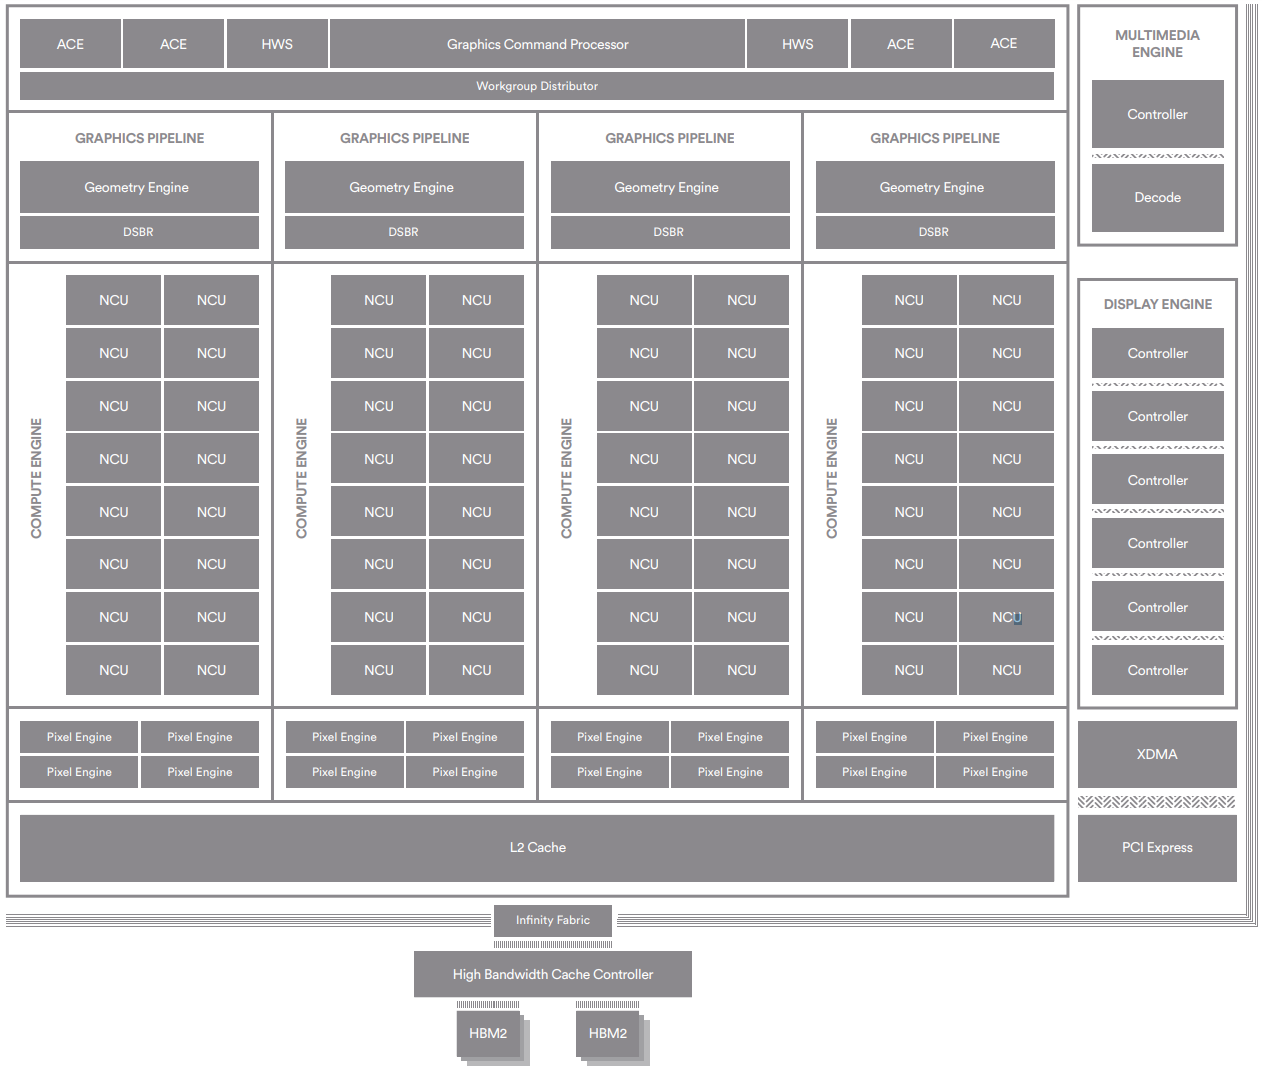
\includegraphics[width=0.7\linewidth]{Figures/Background/Vega10_microarchitecture.png}}
    \subfigure[NCU]{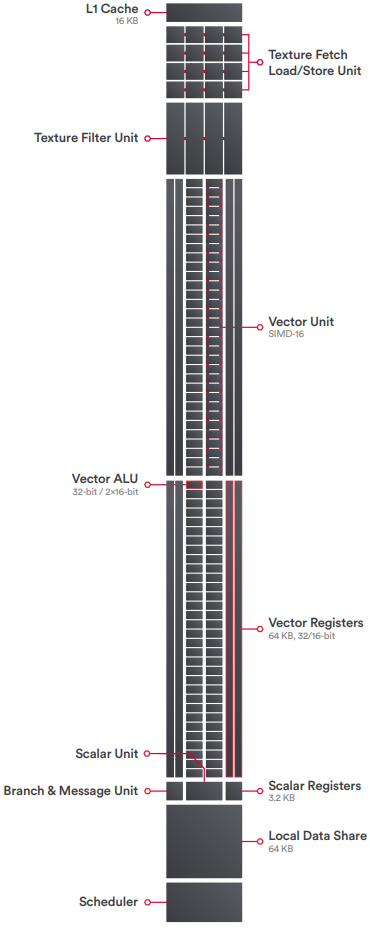
\includegraphics[width=0.24\linewidth]{Figures/Background/NCU.png}}
  \end{subfigmatrix}
  \caption{AMD's Graphics Core Next logical organization.}
  \label{fig:Vega10arch}
\end{figure}


As it was referred before, one of the significant benefits of \acrshort{gpu}s is, the ability to concurrently execute multiple threads. To accomplish for that, each \acrshort{sm} or \acrshort{cu} is made up of hundreds of execution units. However, to manipulate such number of threads, it is necessary to have a significantly large and fast memory system, not only to save the context of each thread, but also to provide low-overhead context switching between the different sets of threads being executed. In that sense, modern \acrshort{gpu} architectures include a large register file on each \acrshort{sm}/\acrshort{cu}. For reference, in the AMD GNC architecture, each \acrshort{cu} has 49,152 (32-bit) registers~\cite{jing_energy-efficient_2013}.

In terms of memory, both the AMD and the NVIDIA \acrshort{gpu}s present a 3 level hierarchy system: a global memory, accessible by all \acrshort{sm}/\acrshort{cu} (generally referred to as video memory); a shared memory associated to each \acrshort{sm} or \acrshort{cu}, accessible by the threads running on that \acrshort{sm} or \acrshort{cu}; and a set of read-only caches for constants and textures, specific to each execution unit.

A \acrshort{gpu} device from AMD will be used to conduct the experimental part of this dissertation. For that reason, the terminology used by AMD will be adopted herein. However, the presented work is independent of the hardware and terminology itself, and could equally be applied to NVIDIA \acrshort{gpu}s.

\subsection{GPU programming model}

The development of CUDA~\cite{nvidia_cuda_2017} (by NVIDIA) and OpenCL~\cite{noauthor_opencl_2013} (by Khronos Group) were the driving force to using \acrshort{gpu}s in general programming. CUDA and OpenCL are both parallel computing platforms and application programming interfaces (\acrshort{api}) that allow developers to create \acrshort{gpu}-accelerated applications, splitting the computations between the \acrshort{cpu} and \acrshort{gpu}. The first versions of these frameworks treated the \acrshort{gpu} as an accelerating slave device, providing a set of directives that allow the \acrshort{cpu} (master device) to transfer data, synchronize and control the \acrshort{gpu}.  Though, to take full advantage of the \acrshort{gpu} architecture and create a true heterogeneous system, the \acrshort{cpu} and \acrshort{gpu} have to collaborate more efficiently. The creation of the Heterogeneous System Architecture (\acrshort{hsa}) \cite{hwu_heterogeneous_2015} framework acts on improving this problem by acting as a low-level intermediary \acrshort{api} to provide improved coordination and communication for heterogeneous computing systems.  More recently, AMD introduced the Radeon Open Computing platform (\acrshort{roc}) \cite{noauthor_radeonopencompute/rocm_2019}. Like CUDA and OpenCL, \acrshort{roc} provides a set of tools that allow developers to create heterogeneous applications. Being a newer software stack, already built on the notions and added benefits of \acrshort{hsa} runtime \acrshort{api}, ROC allows the use of a wider set of programming frameworks like OpenCL, HC++, and HIP.

This programming model is rather similar across the different platforms, with developers traditionally programming the \acrshort{gpu}s using general-purpose languages like C, C++ and Fortran. More recently, the manufacturers are also starting to provide direct access to the \acrshort{gpu} through higher-level languages like Python\footnote{https://developer.nvidia.com/how-to-cuda-python}, allowing for an easier development and adoption of \acrshort{gpu}s as accelerating devices.

Overall, when executing a program on \acrshort{gpu}s, using either of the previously mentioned platforms, a Kernel is invoked on the \acrshort{gpu}, that will execute across several parallel threads. Following this work split, the frameworks expose three levels of abstraction: \textit{threads}, \textit{thread blocks} and  \textit{block grid}. The number of \textit{threads} to be executed can be explicitly defined by the programmer, or implicitly set by the compiler. The \textit{threads} are grouped in \textit{thread blocks} containing an amount of \textit{threads}, and the \textit{thread blocks} are in turn arranged in a \textit{block grid}. When the Kernel is executed, the scheduler maps each \textit{thread block} onto a \acrshort{cu}. Due to this mapping, \textit{threads} within a \textit{thread block} are able to communicate over the \acrshort{cu} shared memory and their execution is synchronized through programable directives.

During the execution of each \textit{thread}, an identifier presents the location of the running \textit{thread} within the \textit{thread blocks} - \texttt{ThreadIdx} and within the \textit{block grid} - \texttt{BlockIdx}. The \textit{thread block} size can be obtained with the \texttt{BlockSize} directive. 

%%%%%%%%%%%%%%%%%%%%%%%%%%%%%%%%%%%%%%%%%%%%%%%%%%%%%%%%%%%%%%%%%%%%%%%%
\section{CMOS Circuit Characterization}
\label{section:CMOS}

For the last 40 years, \acrshort{cmos} (Complementary metal-oxide-semiconductor) has been the most used technology in the creation of digital circuits and processors in general [REF]. 

There are two defined logic levels in digital circuits: logic level $0$ and $1$, each represented by an analog voltage range. To ensure its operations, the circuit requires a DC voltage value $V_{DD}$. The logic gates are excited through an input voltage $V_{i}$ and an output voltage $V_o$, corresponding to the logic level resulting from their logic function (see Figure~\ref{fig:cmos}). As it is illustrated in Figure~\ref{fig:cmos_noise_margin}, the voltage range at the input of the logic gates is correctly interpreted if it falls inside a given range. Logic level $0$ corresponds to the interval between $GND$ ($0V$) to $V_{IL}$, while logic level $1$ corresponds to the interval between $V_{IH}$ to $V_{DD}$. In turn, the output is considered $0$ if it goes from $GND$ ($0V$) to $V_{OL}$ and logic level $1$ from $V_{OH}$ to $V_{DD}$. The limits of the input and output logic levels depend on the intrinsic characteristics of the transistors, such as their dimensions and transconductance values. In addition to the transistors characteristics and operating voltage, any digital circuit is also characterized by their frequency of operation.

\begin{figure}[htb]
    \centering
    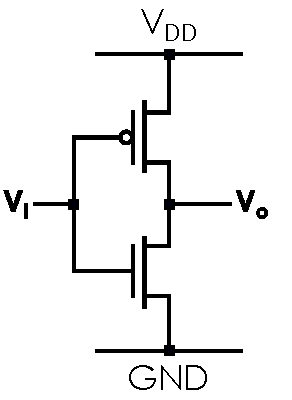
\includegraphics[width=30mm]{Figures/Background/cmos_inverter.pdf}
    \caption{CMOS inverter.}
    \label{fig:cmos}
\end{figure}

\begin{figure}[htb]
    \centering
    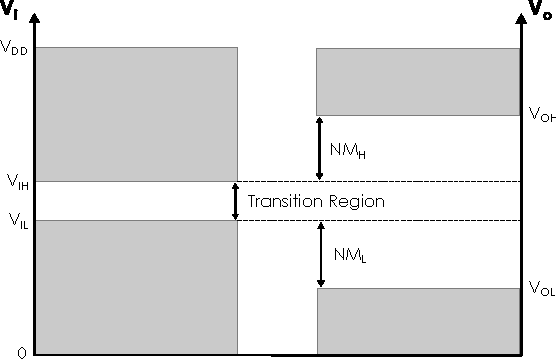
\includegraphics[width=85mm]{Figures/Background/voltage_margin.pdf}
    \caption{Noise margin definitions: $NM_L=V_{IL}-V_{OL}$ and $NM_H=V_{OH}-V_{IH}$.}
    \label{fig:cmos_noise_margin}
\end{figure}

The remaining of this section provides an introduction to the effects of voltage and frequency scaling on the transistor and circuit level operation.

% Moore's law predicted the doubling of the transistors counts roughly every two years. The increase in the number of devices per chip directly translates to the observed performance increase over the last 60 years. However, in the last ten years, the industry is experiencing a slowdown. The shrinking of transistors is harder and harder and the amount of power created by today's chips is limits the transistor count (for the same node size). In this regard, it is indispensable that any digital circuit and, processors in particular, are develop taking into account the underlaying fabrication technology characteristics in order to find new ways of tackling this issues.

% The fundamental solution followed nowadays acts on varying the frequency and voltage values of the CMOS circuit accordingly to what is happening on the device. However, to take fully advantage of these parameters, it is critical to understand the impact of these variations on CMOS circuits.



\subsection{Propagation delay and circuit critical path}

The propagation delay of a logic gate (e.g., inverter) corresponds to the time interval (calculated at $50\%$ of low/high transition) between the application of an input signal and corresponding output switching, as illustrated in Figure~\ref{fig:tp}. Considering both transitions low to high and high to low, the logic gate propagation time ($tp$) corresponds to the average value of the two propagation delays, as defined in Equation~\ref{eq:tp_avg}.

\begin{figure}[htb]
    \centering
    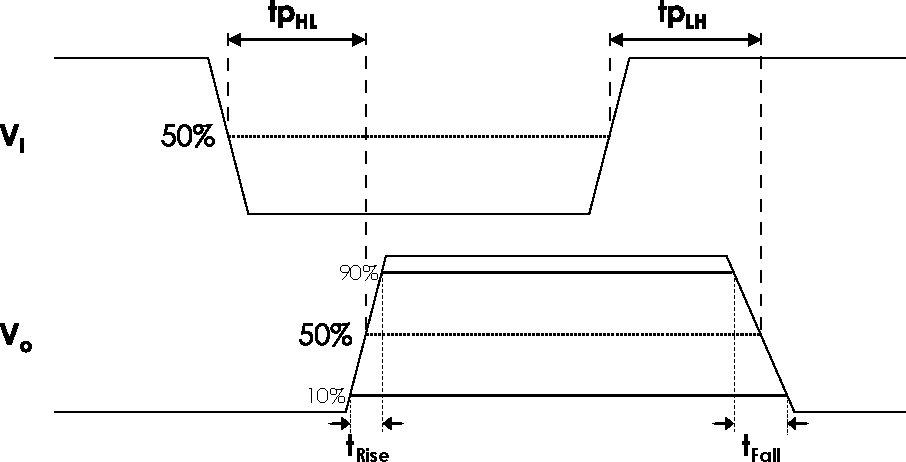
\includegraphics[width=80mm]{Figures/Background/propagation_delay.pdf}
    \caption{Logic gate propagation delay: $tp_{HL}$ - propagation delay high to low; $tp_{LH}$ - propagation delay low to high.}
    \label{fig:tp}
\end{figure}

\begin{equation}
    tp = tp_{avg} = \frac{tp_{HL}+tp_{LH}}{2}
    \label{eq:tp_avg}
\end{equation}

This metric is related to the time that the logic gate takes to switch its output logic level ($t_{Fall}$ for the high to low transition and $t_{Rise}$ for the low to high transition). This transition can be modeled as a first-order RC circuit (see Figure~\ref{fig:rc_circuit}) with the transient response following Equation~\ref{eq:firtst_order}, where $\tau$ corresponds to the time constant. This time constant reflects the intrinsic characteristics of the transistors that make up the logic gate, being $\tau=RC$, where $R$ represents the average output resistance of the transistor when it is turned 'ON' and $C$ the output capacitance that the logic gate is driving.


\begin{figure}[htb]
    \centering
    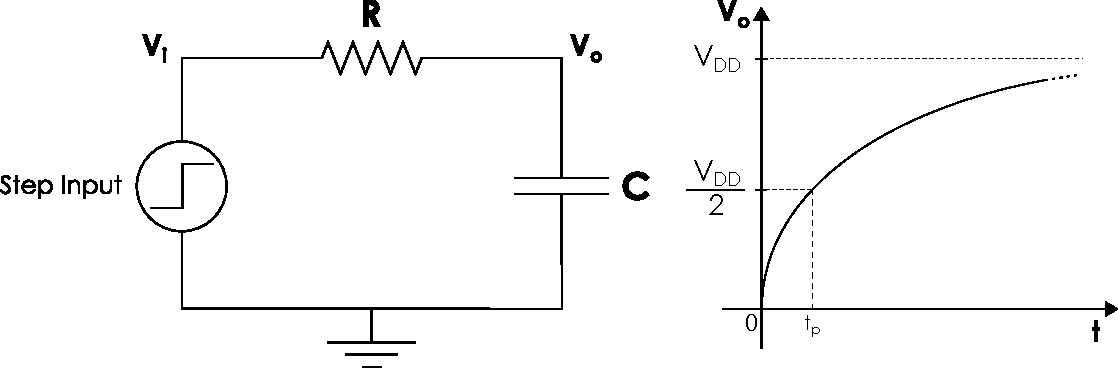
\includegraphics[width=105mm]{Figures/Background/rc_circuit.pdf}
    \caption{First order RC circuit and its corresponding temporal response to step input.}
    \label{fig:rc_circuit}
\end{figure}

\begin{equation}
    V_o=V_{DD} \cdot (1-e^{-t/\tau})
    \label{eq:firtst_order}
\end{equation}

By solving Equation~\ref{eq:firtst_order} for $V_o=\frac{V_{DD}}{2}$, it is observed that the propagation delay is a function of the supplied voltage, of $R$ and $C$, as depicted in Equation~\ref{eq:tp}.


\begin{equation}
    t_p=-ln\left(1-\frac{V_{DD}}{2 \cdot V_{DD}}\right)\cdot\tau=-ln(0.5)\cdot\tau=ln(2)\cdot\tau
    \label{eq:tp}
\end{equation}


From all the logic paths (sequence of logic gates) that connect any two registers, the one which presents the largest sum of the propagation delay limits the overall maximum frequency that the \acrshort{cmos} circuit can operate, establishing itself as the critical path of the circuit (see Figure~\ref{fig:critical_path}). However, in the particular case of a microprocessor circuit, depending on the operation (instruction) being performed (and so, of the used architectural component), the circuit's critical path can change.

\begin{figure}[htb]
    \centering
    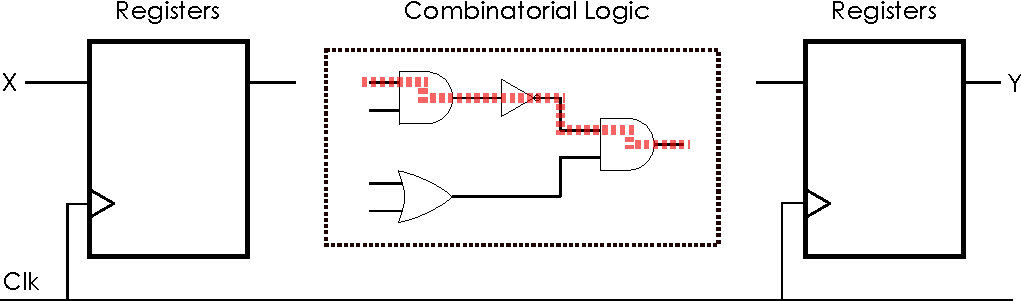
\includegraphics[width=130mm]{Figures/Background/comb_logic.pdf}
    \caption{Critical path between two registers (red dashed line).}
    \label{fig:critical_path}
\end{figure}

In this way, when scaling the circuit's operating frequency, it is only possible to increase it until it matches the inverse of the critical path propagation delay. When raising the frequency ahead of this value, the critical path is violated, meaning that when the next clock cycle starts, the output of the combinatorial logic may not be the correct one.

% When manufacturers set the digital circuit's operating frequency, they never go up to the maximum possible frequency, leaving a safe operating margin. This margin exists to guarantee correct and safe operation under process, voltage and temperature (\acrshort{pvt}) variation.



\subsection{Voltage guardband, PVT Variation and Aging}

After the release of the digital circuit, silicon vendors often deal with variations of their devices' specifications. On the design stage of the circuit, these variations need to be correctly predicted and accounted for, guaranteeing the correct operation of the circuit throughout time and range of conditions that the circuit will be exposed to.

Process, voltage and temperature (\acrshort{pvt}) variation and aging impact the circuit in different manners and the solution for all is to put in place a voltage guardband, as defined in Figure~\ref{fig:voltage_guardband}. This voltage guardband increases the circuit nominal voltage from the best-case operating voltage selected from the transistors and gates' intrinsic characteristics.
In Equation~\ref{eq:tp}, the propagation delay is now obtained by considering the ratio between the best-case operating voltage\footnote{(Threshold voltage) and the considered supply voltage}. Hence, when the silicon vendor opts to put in place a voltage guardband, increasing the supplied voltage (overvoltage), the propagation delay will follow Equation~\ref{eq:tp_v_scaling}, where $V_{Threshold}$ depends on the transistors (and so, it does not depend on the supply voltage value) and $V_{Supply \: Voltage}$ is the supplier controlled parameter. Figure~\ref{fig:voltage_scaling} illustrates the logic gate step response for over and undervoltage. Increasing the supply voltage will make the transistors switch faster, while decreasing it, reduces the switching pace.



\begin{equation}
    t_p=-ln \left( 1-\frac{V_{Threshold}}{V_{Supply \: Voltage}}\right)\cdot\tau=ln\left(\frac{2V_{Supply \: Voltage}}{2V_{Supply \: Voltage}-V_{Threshold}}\right)\cdot\tau
    \label{eq:tp_v_scaling}
\end{equation}

\begin{figure}[!htb]
    \centering
  \begin{subfigmatrix}{2}
    \subfigure[Voltage guardband definition.]{
    \centering
    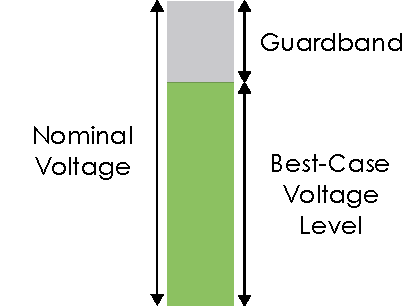
\includegraphics[height=4cm]{Figures/Background/voltage_guardband_bar.pdf}
    \label{fig:voltage_guardband}}
    \subfigure[First order circuit step response when changing the supply voltage ($V_{sv}$).]{
    \centering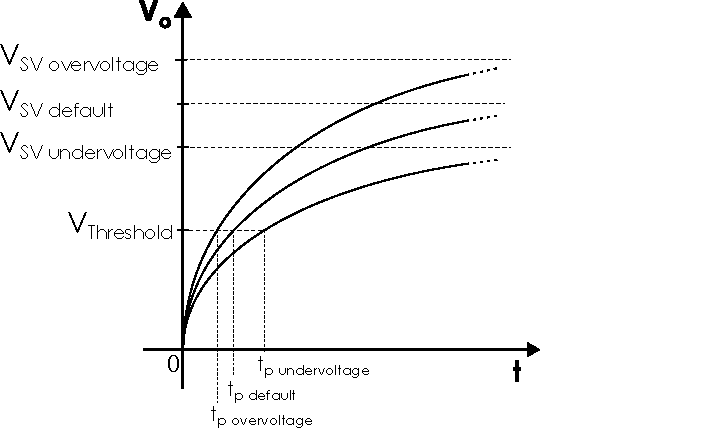
\includegraphics[height=7cm]{Figures/Background/v_scaling.pdf}
    
    \label{fig:voltage_scaling}}
  \end{subfigmatrix}
  \caption{Voltage guardband ensures reliability by making the transistors switching faster.}
\end{figure}




\subsubsection{Process variation and aging}

Process variation and aging impact the circuit in different ways. Process variation is related to the modern fabrication process of silicon. It results from imperfections in the lithography and dopant diffusion, affecting the transistors' dimensions (for example, length and oxide thickness). This dimensionality change between the transistors can occur either intra-die, when devices from the same die present different features depending on their locations, and inter-die, meaning that devices from one die can present different traits from devices from another batch of dies. The process variation affects the speed of transistors and the overall circuit characteristics, by varying the device voltage threshold and speed \cite{schemmert_threshold-voltage_1974, thomas_core_2016}. Such variations are inherent to the fabrication process. Even though silicon manufacturers try to reduce this impact, such variation will always occur as a \textit{static} variation after the release of the chip to the market.

Aging of the \acrshort{cmos} circuits is a result of ongoing chip temperature variation and supply voltage change. The continuous variation of these two factors induces \textit{Bias Temperature Instability} (\acrshort{bti}) and  \textit{Hot Carrier Injection} (\acrshort{hci}). \acrshort{bti} causes threshold voltage shifts over long periods due to the presence of voltage stress at the transistors' gate. On the other side, \acrshort{hci} is caused by the acceleration of carriers (electrons/holes) under lateral electric fields in the channel of MOS devices. The acceleration can get up to the point where the carriers gain enough energy and momentum to cause damage, degrading mobilities and again, changing the threshold voltages~\cite{sapatnekar_what_nodate}.

The occurrence of these phenomenons raises the possibility of the circuit diverge from its original specifications. Hence, a circuit that is dimensioned without any headroom (not sufficiently large voltage guardband) may not be able to cope with such a process variation - producing a not working circuit; or stopping to work overtime due to aging.



\subsubsection{Voltage variation}

As it was previously observed, running the circuit at an increased voltage compared to the required voltage at the target frequency for typical workloads results in a faster circuit. This increment in performance allows for inserting an extra timing margin in each clock cycle, as described in Figure~\ref{fig:timming_guardband}. 

\begin{figure}[!htb]
  \begin{subfigmatrix}{2}
    \subfigure[Static Margin]{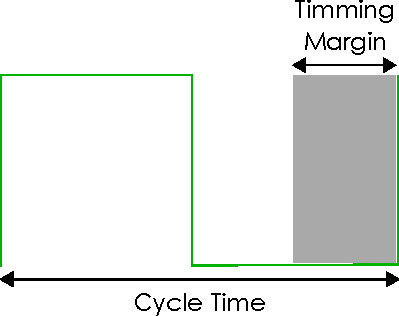
\includegraphics[height=4.5cm]{Figures/Background/static_margin.pdf}}
    \subfigure[Reduced Voltage Margin]{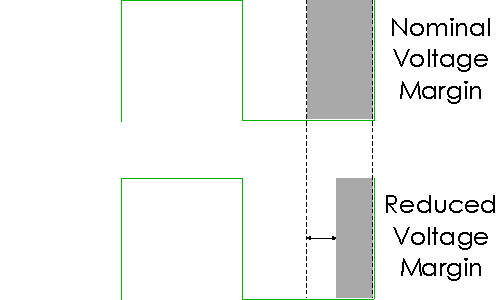
\includegraphics[height=4.5cm]{Figures/Background/reduced_voltage_margin.pdf}}
  \end{subfigmatrix}
  \caption{Voltage guardband ensures operation reliability by effectively inserting some extra timing margin.}
  \label{fig:timming_guardband}
\end{figure}

This timing margin is of extreme importance to cope with voltage noise, the leading cause of voltage variation during the circuit execution. Voltage noise is mainly induced by $di/dt$ droop. This phenomenon makes the actual measured voltage that is  applied to the circuit components (as formulated in Equation \ref{eq:Vactual}), depend on the rate of change of the current being drawn. 

\begin{equation}
    \label{eq:Vactual}
    V_{actual} = V_{DD}-L*\frac{di}{dt}
\end{equation}

The runtime workload intensity variation induces the $di/dt$ droop due to the rapid and significant change in current demand from the various circuit functional blocks~\cite{thomas_core_2016}. Thus, in the case of processors, the workload type can directly impact voltage noise. As a result, a program that induces a bigger $di/dt$ droop will need to have a bigger voltage guardband.

\subsubsection{Temperature variation}

Temperature variation occurs both due to changes on the environmental temperature, and due to changes in the temperature that is dissipated as heat by the transistors on the circuit. The temperature affects the transistors by changing the carriers' mobility ($ \mu [\frac{cm^2}{V\cdot s}]$), and threshold voltage ($V_t$)\cite{wolpert_temperature_2012}.

The carriers' mobility $ \mu $ describes the drift velocity of a particle in an applied electric field, thus the transistor's capability to drive electric current. Usually, the carrier mobility of MOS transistors presents a very complex temperature dependence. However, in general, the mobility is said to decrease with temperature increase. 

In the case of threshold voltage, its rate of change also follows the same principle of the carriers mobility. However, it usually has a more straightforward dependency of decreasing linearly with temperature increase.

The work of Freijado \textit{et al.}~\cite{freijedo_modeling_2012} presents a model that tries to encompass all these variations and test the impact that temperature has on the propagation delay. The designed model predicts that the propagation delay increases linearly with the temperature increase, which would imply that the size of the voltage guardband reduces when the temperature increases. 

\subsection{Power Consumption}
\label{sec:power_consumption}
On a \acrshort{cmos} circuit, the total consumed power is decomposed into the dynamic and static parts

\begin{equation}
    P_{CMOS} = P_{dynamic} + P_{static}.
    \label{eq:power}
\end{equation}

The dynamic power relates to the power that is consumed by the transistors flipping stages (inverting the logic values), and corresponds to the power of charging and discharging the internal net capacitances. This value is proportional to the frequency that this change occurs. Equation~\ref{eq:dynpower} represents the general formulation of the dynamic power, where $a$ represents the device utilization factor, $C$ the total capacitance of the circuit, $V$ the circuit supply voltage, and $f$ the frequency of operation~\cite{gonzalez_supply_1997}.

\begin{equation}
    P_{dynamic} = aCV^2f
    \label{eq:dynpower}
\end{equation}

On the other hand, the static part of the power consumption comprehends three components: $P_{leakage}$, $P_{short-circuit}$ and $P_{DC}$~\cite{mei_survey_2016}. The leakage power is independent of the transistors flip, and it represents the flow of electrons between the transistors' source, drain, and gate, known as leakage current. The short-circuit power comes from the instantaneous short-circuit connection between the supply voltage and the ground when the transistor flips. Finally, the Direct Current (DC) power corresponds to the power needed for powering the circuit. Equation \ref{eq:cmosstatic} represents the expression with all static power consumption components.

\begin{equation}
    P_{static} = P_{leakage} + P_{short-circuit} + P_{DC}
    \label{eq:cmosstatic}
\end{equation}

Usually, the dynamic power dominates the total power consumption of a circuit. However, with the current tendency to reduce the manufacturing size of transistors, the static power is becoming a more significant part \cite{s._hong_modeling_2012,hong_integrated_2010}. Nevertheless, as a common reference, and due to the usually dominant weight of the dynamic power on the total power consumption, the power used by a \acrshort{cmos} circuit usually changes linearly with the clock frequency and quadratically with the supplied voltage.


%%%%%%%%%%%%%%%%%%%%%%%%%%%%%%%%%%%%%%%%%%%%%%%%%%%%%%%%%%%%%%%%%%%%%%%%
\section{Dynamic Voltage and Frequency Scaling}
\label{section:DVFS}

The widespread use of \acrshort{gpu}s in both supercomputers and personal computing machines comes at the cost of a significant increase in power consumption. While a typical modern CPU consumes about 50 to 100W, it is common to see \acrshort{gpu}s consuming between 200 and 300W of power. With these figures, the use of energy efficiency techniques to try to reduce power consumption becomes a vital issue.

As stated in Section~\ref{sec:power_consumption}, the power consumption of a \acrshort{cmos} circuit increases linearly with the operating frequency and quadratically with the supplied voltage. Thus, a direct manner of reducing this figure is by directly acting on these two parameters. A common approach of achieving this is the application of 
Dynamic Voltage and Frequency Scaling (\acrshort{dvfs}), consisting on a power management technique which performs "on the fly" control of frequency and voltage. In particular,\acrshort{dvfs} allows for an energy efficiency improvement by matching voltage and frequency settings to the \acrshort{gpu} utilization. When the \acrshort{gpu} is idle, the frequency is lowered, and when it is active, the frequency is increased. As presented in the previous section, the frequency scaling also implies a consequent change in voltage, to accommodate the fulfillment of the critical path timing constraints. 

In general, the applied voltage level $V$ is a function of the current operating frequency $f$, in the form of $V(f)$. However, by properly controlling the clock frequency, the required voltage level for stable operation of the circuit can also be maintained or even reduced, leading to further power savings.

In general, modern \acrshort{gpu} boards offer an independent control over two pairs of frequency and voltage. Each pair (or domain) acts on a distinct part of the \acrshort{gpu}, intending to maximize the performance or reduce the power consumption. The first domain concerns the \acrshort{gpu} core, acting on all \acrshort{sm}/\acrshort{cu}s, the cache, and the interconnection fabric. The second affects the \acrshort{dram} chips that compose the video memory. 

The clock frequency is an independently controlled variable, and its change directly reflects on the performance that is achieved by the \acrshort{gpu}. An increase in the clock frequency of the core results in an improvement of the \acrshort{sm}/\acrshort{cu} execution speed, while the same change in the memory frequency will increase the \acrshort{dram} I/O throughput \cite{mei_survey_2016}. The voltage level of each domain is dependent on the clock frequency being used and it is usually defined based on tests performed by the manufacturer to ensure the correct operation of the circuit, independently of the workload.

The two major \acrshort{gpu} silicon vendors, AMD and NVIDIA, adopted the concept of performance levels on their products. Each performance level is a pair of frequency and voltage that can be applied to each \acrshort{gpu} \acrshort{dvfs} domains. These vary from low power and performance levels to high power and performance ones. The idea of having multiple performance levels is to allow the application to have the best point of operation. In the case of the first \acrshort{gpu} device (AMD Vega 10 Frontier Edition) that is going to be used in the experimental phase of this dissertation, the \acrshort{gpu} core has eight performance levels, while the memory has only four. Table \ref{tab:gpulevels} shows the reference values (for the pairs of frequency and voltage) for each of the core and memory performance levels. 
The frequency and voltage of higher performance levels reflect the expected behaviour, with an increase of the supply voltage to accommodate the frequency boost.


\begin{table}[!htb]
\renewcommand{\arraystretch}{1.2} % more space between rows
\centering
\begin{tabular}{ccclccc}
\multicolumn{3}{c}{\textbf{Core}}                                         & \multicolumn{1}{c}{\textbf{}} & \multicolumn{3}{c}{\textbf{Memory}}                                             \\
\textbf{Level} & \textbf{Frequency {[}MHz{]}} & \textbf{Voltage {[}mV{]}} &                               & \textbf{Level}       & \textbf{Frequency {[}MHz{]}} & \textbf{Voltage {[}mV{]}} \\ \cline{1-3} \cline{5-7} 
0              & 852                          & 800                       &                               & 0                    & 167                          & 800                       \\
1              & 991                          & 900                       &                               & 1                    & 500                          & 900                       \\
2              & 1138                         & 950                       &                               & 2                    & 800                          & 950                       \\
3              & 1269                         & 1000                      &                               & 3                    & 945                          & 1000                      \\ \cline{5-7} 
4              & 1348                         & 1050                      &                               & \multicolumn{1}{l}{} & \multicolumn{1}{l}{}         & \multicolumn{1}{l}{}      \\
5              & 1440                         & 1100                      &                               & \multicolumn{1}{l}{} & \multicolumn{1}{l}{}         & \multicolumn{1}{l}{}      \\
6              & 1528                         & 1150                      &                               & \multicolumn{1}{l}{} & \multicolumn{1}{l}{}         & \multicolumn{1}{l}{}      \\
7              & 1600                         & 1200                      &                               & \multicolumn{1}{l}{} & \multicolumn{1}{l}{}         & \multicolumn{1}{l}{}      \\ \cline{1-3}
\end{tabular}
\caption{GPU core and memory performance levels for the AMD Vega 10 Frontier Edition GPU.}
\label{tab:gpulevels}
\end{table}


Newer \acrshort{gpu} \acrshort{dvfs} systems, like the one used on the second \acrshort{gpu} under test (AMD Radeon 5700 XT) improve the number of performance levels by allowing for a continuous used of all frequency values within the valid range (versus discretizing the domain into a set number of performance levels). In this case, there are three user-defined frequency-voltage pairs on which a quadratic regression is computed  (see Figure~\ref{fig:voltage_curve}), creating a $f(V)$ function that for every frequency, gives the correspondent voltage value.

\begin{figure}[htb]
  \centering
  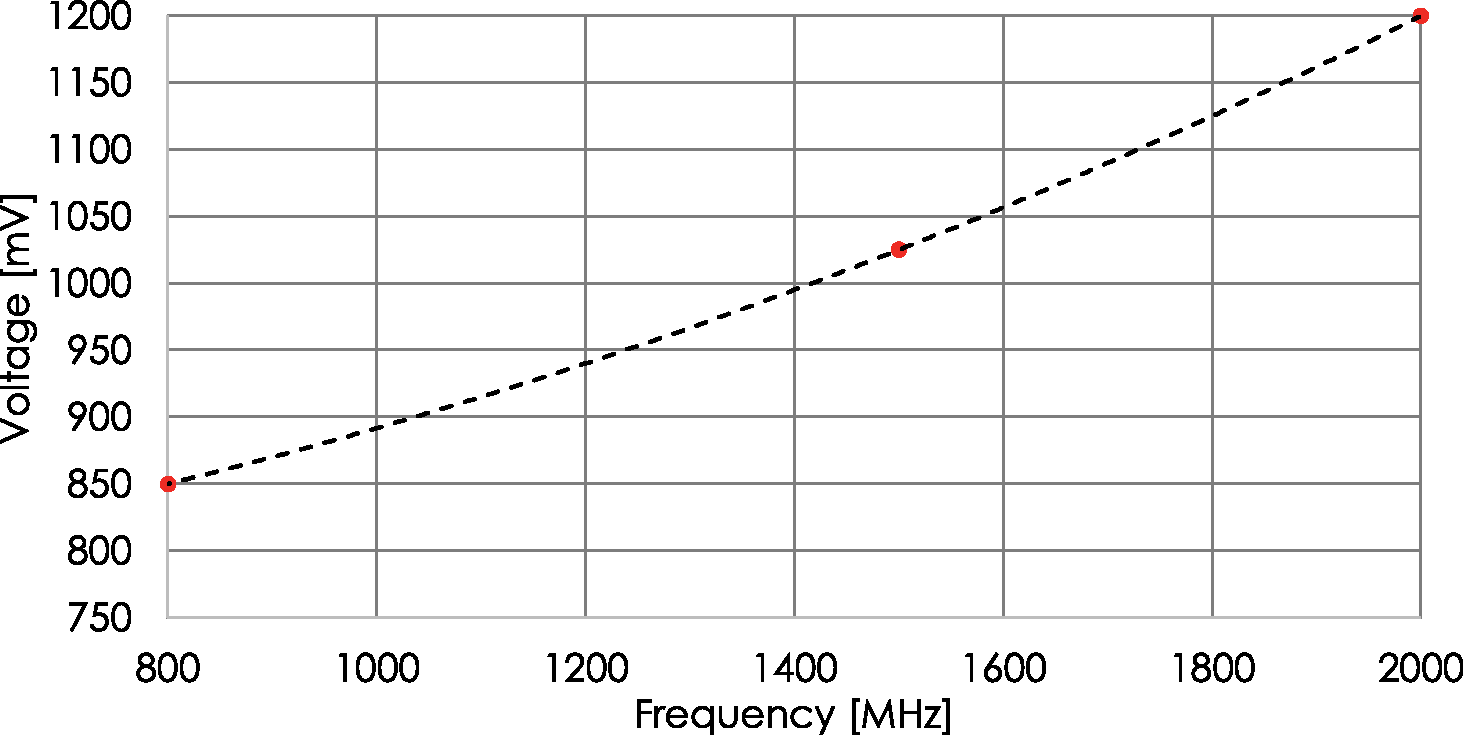
\includegraphics[width=0.75\textwidth]{Figures/Background/voltage_frequency_curve.pdf}
  \caption{GPU Core voltage frequency curve, red dots indicate the default user-defined voltage frequency pair - AMD Radeon 5700 XT.}
  \label{fig:voltage_curve}
\end{figure}

\subsection{Control Mechanism}

The correct choice of the most appropriate performance level for each \acrshort{gpu} \acrshort{dvfs} domain when executing a given application is one of the topics that has deserved a special attention from both manufacturers and researchers, since the design of the \acrshort{dvfs} controller has a significant impact on the \acrshort{gpu}'s performance and energy efficiency.

The first implementations of \acrshort{gpu} \acrshort{dvfs} controllers took a direct inspiration from the \acrshort{cpu} \acrshort{dvfs} controllers and can be largely classified into interval-based, inter-task, and intra-task \acrshort{dvfs} schemes~\cite{boyer_improving_2013}. 

\subsubsection{Interval-based}

Interval-based algorithms rely on the periodical measurement of the device's utilization, setting the next frequency and voltage levels based on the average measurement of utilization. The utilization $U_{i}$ reflects the percentage of working time, $w_{i}$, that was spent by the \acrshort{gpu} over the last time frame $TF_{i}$ and can be formulated using equation \ref{eq:utilization}.

\begin{equation}
    U_i=\frac{w_i}{TF_i}
    \label{eq:utilization}
\end{equation}

By applying either a arithmetic, a geometric, a weighted average, or even a more complex metric over the last $n$  measurements,  the next utilization $U_{i+1}$ is predicted. If the predicted value surpasses pre-determined upper or lower thresholds, the frequency is adjusted up or down accordingly \cite{seongki_gpgpu-perf:_2015}. 
A \textit{governor} is a set of parameters (such as frequency and voltage tables), thresholds and a utilization prediction algorithm that controls how the interval-based \acrshort{dvfs} works. By choosing a different \textit{governor}, the \acrshort{dvfs} system can react differently to the same workload. Figure \ref{fig:DVFSprocedure} schematizes the periodic procedure executed by the \acrshort{dvfs} system~\cite{seongki_gpgpu-perf:_2015}. 

\begin{figure}[htb]
  \centering
  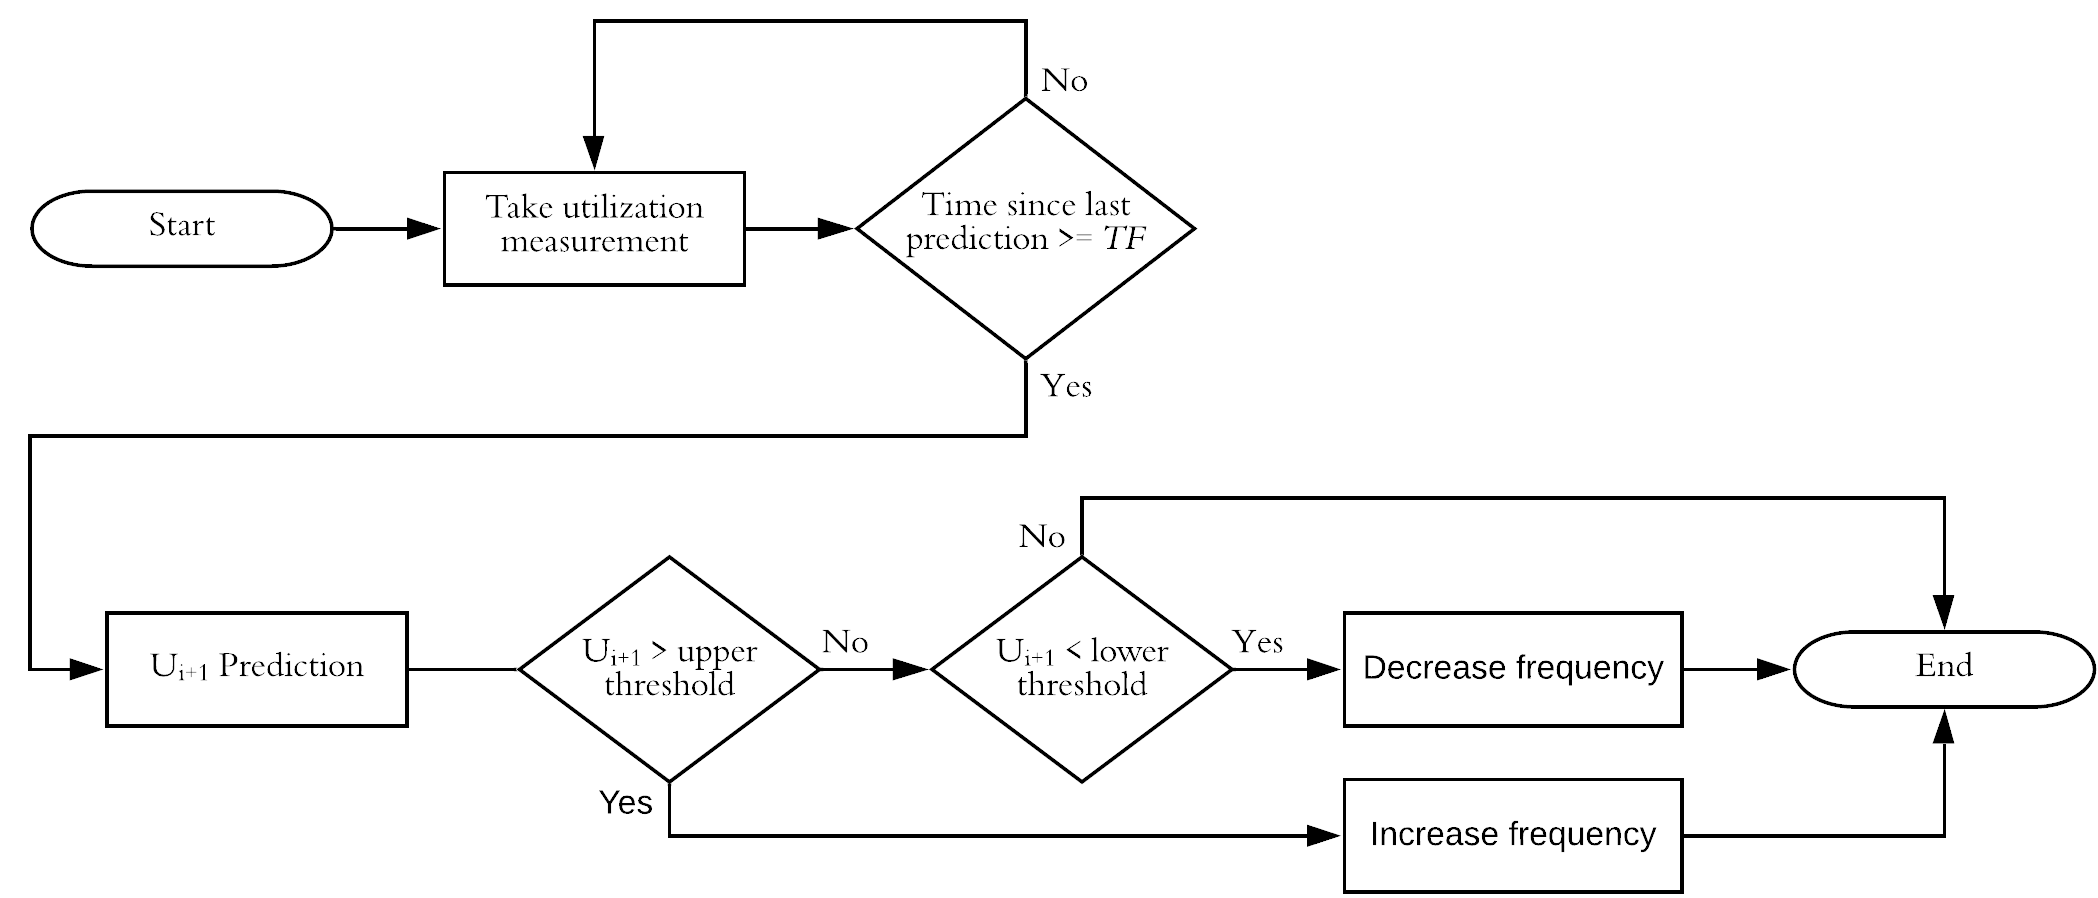
\includegraphics[width=\textwidth]{Figures/Background/DVFSprogram.png}
  \caption{Interval-based DVFS procedure.}
  \label{fig:DVFSprocedure}
\end{figure}

\subsubsection{Inter/Intra task-based}

The Inter and Intra task-based \acrshort{dvfs} algorithms analyze the program source code, as well as some past runs profiling results to determine the optimal frequency/voltage for each task. This type of algorithm is composed of an intra-task and an inter-task analysis \cite{noauthor_time_nodate}. The intra-task part decomposes the process execution into the on-chip computation and off-chip access latencies. Based on the results,  the optimal \acrshort{gpu} core and memory frequencies are determined accordingly to the ratio between the two types of execution. Inter-task mechanisms utilize the intra-task results, assigning a signature to each type of task/process. By analyzing, in run-time, the \acrshort{gpu} components' utilization, and using a lookup table that stores the signatures, the optimal frequency/voltage is selected for the sequence of tasks to be executed.

In general, the challenges of creating a better \acrshort{gpu} \acrshort{dvfs} mechanism relates to three factors: \acrshort{gpu} power management, \acrshort{dvfs} performance and power estimation tools and continuous changing architecture. 
The current \acrshort{gpu} devices deliver minimal and simplified power management mechanism, solely relying on controlling the device power cap. The complete architectural renew that happens on each \acrshort{gpu} generation does not allow for the creation and maturation of accurate quantitative \acrshort{gpu} \acrshort{dvfs} performance and power estimation tools. 
And again, the complete redo of the architecture on each generation also makes the energy efficiency strategies applied to one architecture design have different outcomes on the next one~\cite{mei_survey_2016}. The observed results show that strategies like scaling up the processor frequency, race-to-idle  \cite{hoffmann_racing_2013} or "racing" \cite{kim_racing_2015}, when a task is launched in the pursuit of finishing it as fast as possible and return to an idle state, prof to increase the energy efficiency of CPUs. However, that assumption not always results in the same outcome for \acrshort{gpu}s \cite{kim_racing_2015}. 

\subsubsection{AMD/NVIDIA DVFS Mechanism Example}

The \acrshort{gpu} \acrshort{dvfs} control mechanism that is used nowadays by both AMD and NVIDIA, schematized in figure \ref{fig:DVFSmechanism}, is primarily an interval-based one. In particular, the most recent AMD \acrshort{gpu} \acrshort{dvfs} mechanism is called Adaptive Frequency and Voltage Scaling (\acrshort{afvs}) \cite{amd_polaris_2017}. It takes into account the voltage levels across the different parts of the \acrshort{gpu}, the die temperature, the desired frequency and the total power consumption. In order to maintain the total power consumption within the required power and temperature envelope. Upon launching a new task and within a set power target, the \acrshort{gpu} tries to achieve the highest possible frequency (or highest performance level). For that frequency configuration, it also adjusts the voltage level to the one required to ensure the correct operation. Naturally, with the highest performance level, power and temperature will increase. When one of these parameters achieves the limit, the \acrshort{gpu} decreases the frequency (or selecting a more energy-saving performance level) to maintain itself within the power and temperature target. 

\begin{figure}[htb]
  \centering
  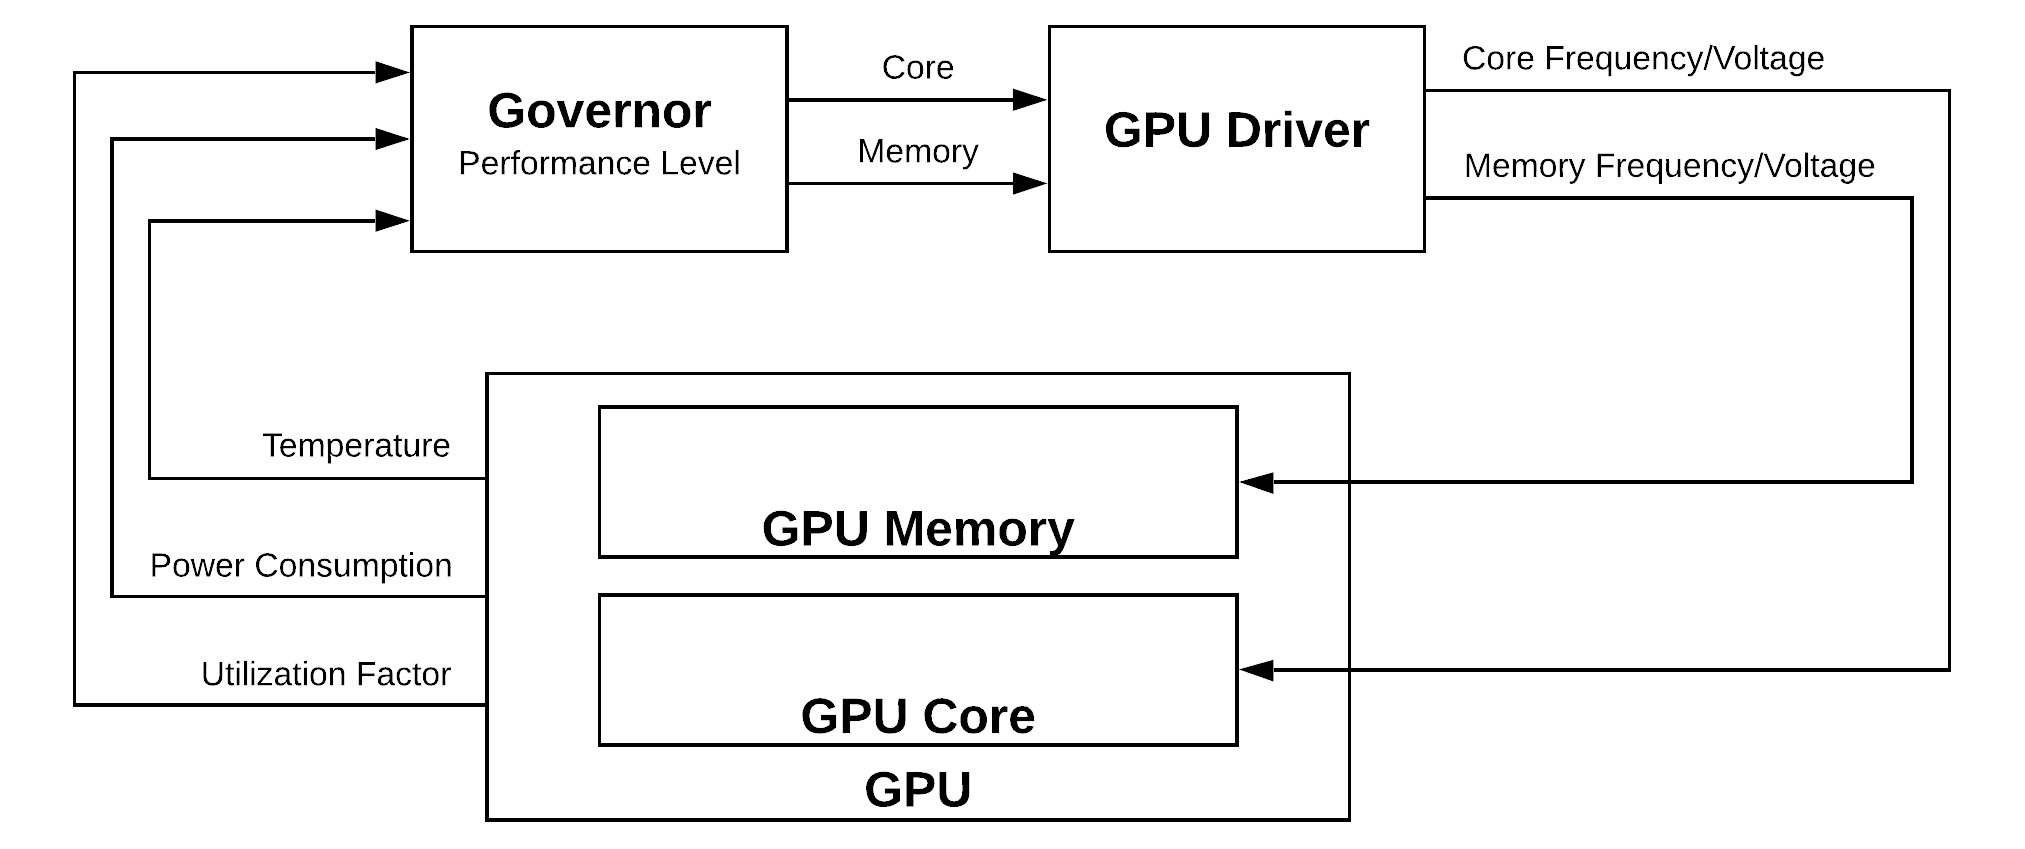
\includegraphics[width=0.8\textwidth]{Figures/Background/DVFS.png}
  \caption{AMD/NVIDIA DVFS control mechanism.}
  \label{fig:DVFSmechanism}
\end{figure}

The major drawback of current \acrshort{gpu} \acrshort{dvfs} implementations is not taking into account the type of tasks that the \acrshort{gpu} is executing. The dominant control mechanism still considers the \acrshort{gpu} as a black box and controls its \acrshort{dvfs} settings by only looking at outside parameters. Even though such a black-box approach enables significant improvements in current hardware, it lacks the optimization of the frequency/voltage to the type of workload. For instance, a given application can be either compute-bound or memory-bound, depending on if the time that it takes to perform the task is limited by the processor performance or by the memory bandwidth and latency. This binary classification of applications also depends on the frequency of the core and memory. The same application can be compute-bounded at a low core frequency but be memory-bounded at a higher one \cite{guerreiro_dvfs-aware_2019} (the bottleneck switches from the processing elements to the memory). In the case of a compute-bounded application, the limitation can be imposed by different components of the processor architecture, depend on the type of data (integer or floats) and on the intended precision (size of the operands). If one compares the computation with the same type of operands, but with different precision (for instance, 16 vs. 32 bits), even though the \acrshort{gpu} uses the same arithmetic unit, the critical path for 32 bits operands is of increased length. Hence, the maximum delay between the input and the operations output increases with the operands' precision. 
Since no information about the application is provided to the \acrshort{dvfs} controller, no adaptation of the V-F settings can be employed.
Considering that the manufacturers do not usually tune their devices to the minimum voltage level (to accommodate for manufacturing imprecisions and to leave a safe guardband), there is some space to reduce the operating voltage of the circuits, leading to significant power savings. 

Overall, the minimum operating voltage of each performance level is set at a high enough level to ensure the correct operation of the \acrshort{gpu}, independently of the type of computations/workload. Nevertheless, it is possible to further fine-tune the voltage and frequency configuration if the type of task being executed is known at run-time.Furthermore, a significant limitation of the voltage-frequency control system is the time it takes to change and stabilize the intended V-F pair. On the case on the AMD Vega 10 Frontier Edition, the mechanism takes approximately 200-500 ms to change between performance levels.

\subsection{GPU DVFS Characterization}

To improve the performance and energy efficiency of a \acrshort{gpu}, it is important to characterize and analyze the effects of applying \acrshort{dvfs} techniques on its operation, with a special emphasis in what concerns the impact of the different parameters on different workload scenarios. 

A complete \acrshort{gpu} \acrshort{dvfs} characterization is explored in the literature using two methodologies. The first refers to experimental studies, where researchers use real \acrshort{gpu}s to perform voltage and frequency scaling. However, due to past dominance of NVIDIA over AMD \cite{noauthor_jon_2018, mujtaba_amd_2019} and the fact that this manufacturer only offers limited support for independent voltage scaling tools, the majority of the work act solely on frequency scaling. The second approach uses simulators, like GPGPU-Sim \cite{noauthor_gpgpu-sim/gpgpu-sim_distribution_2019} and GPUWattch \cite{noauthor_gpu_2011, leng_gpuwattch:_2013},  to simulate various scaling approaches, like \acrshort{gpu} core number scaling and per-core \acrshort{dvfs} \cite{mei_survey_2016}. The benefit of using simulators over real hardware comes on the increased flexibility, enabling the experimentation of scenarios not supported by the frequency/voltage scaling tools provided by the manufacturers. In both methodologies, the studies act on the impact on performance, energy consumption and overall energy efficiency.

The following subsections present a brief overview of some of these works.


\subsubsection{Experimental Approach}

Jiao \textit{et al.}~\cite{jiao_power_2010} scaled the \acrshort{gpu} core and memory frequencies of an NVIDIA Tesla GTX 280 \acrshort{gpu} using three types of workload: a compute-bounded dense matrix multiplication application; a memory bounded application that performs a dense matrix transpose; and a mixed workload, executing a Fast Fourier Transform (FFT) computation. The experimental study showed that for the same core-memory frequency settings, the three applications showed different performance and energy efficiency curves. While a compute bounded application showed to be insensitive to memory frequency scaling, the memory bounded application takes advantage of high memory frequency and low core frequency. At last, the mixed workload FFT application profits from both high core and memory frequency. In general, it was also shown that energy efficiency could be determined by the instructions per cycle (IPC) metric and by the global ratio of memory transactions by computation transactions.

Ge \textit{et al.} \cite{ge_effects_2013} explored dense matrix multiplication kernel executions in more detail using an NVIDIA Kepler K20c \acrshort{gpu}.  The conducted work revealed that for this type of kernel (compute-bounded), the \acrshort{gpu}'s power and achievable performance is linear to the \acrshort{gpu} core frequency and that the total energy consumption had no relation to frequency scaling. In all the used application tests, the energy efficiency has a linear relation with the \acrshort{gpu} frequency, with the highest energy efficiency being achieved when the highest clock frequency was employed.

Abe \textit{et al.} \cite{abe_power_2012} introduced a global scaling procedure that combines the \acrshort{gpu} core and memory frequency with the host \acrshort{cpu} frequency, in order to minimize the energy consumption. The first experiment tried to optimize the computation of dense matrix multiplication with different matrix sizes. By using this global scheme on a small matrix leads to a 28\% energy saving, when using low \acrshort{gpu} memory frequency and high \acrshort{gpu} core frequency. The same procedure was then enlarged to a more diverse set of 33 benchmarks, where all the possible combinations of a low, medium, and high \acrshort{gpu} core and memory frequencies were tested to find the optimal working settings. It was found that energy consumption can be reduced as much as 75\% with a performance loss of 30\% when the best settings were used. 

Mei \textit{et al.} \cite{mei_measurement_2013} conducted a more general experimentation using 37 \acrshort{gpu} benchmarks. In this work, it was possible to observe that the effect of \acrshort{gpu} \acrshort{dvfs} depends on the application characteristics. In all situations, the fine-tuning of \acrshort{dvfs} per application (finding the lowest voltage level for the desired running frequency) conveyed an energy-saving of 20\%, on average, with only a 4\% performance loss. More recently, Mei  \textit{et al.}, expanded the previous work to analyze the relation between energy consumption and dynamic frequency scaling settings \cite{mei_survey_2016}. For the  Rodinia benchmark \cite{che_rodinia:_2009}, it was found that some benchmarks increase the energy consumption linearly with frequency scaling while others are insensitive to the change of this parameter. In the particular case of \acrshort{gpu} memory frequency scaling, the work revealed that underclocking this component can result in a 30\% energy decrease if the running application is not memory bounded. For the case of applications whose performance depends on the memory, decreasing its frequency can lead up to 54\% energy increase, mostly due to the increased execution time. The tested set of applications showed that overclocking the memory results in diminishing the execution time with reduced overall energy consumption (the memory energy consumption increase overshadows the small reduction in computation time). 

Overall, the relation between the \acrshort{dvfs} settings and the resulting energy consumption depends heavily on the application type. One can conclude that a simple linear model (normally used by the \acrshort{gpu} manufacturers) for \acrshort{dvfs} settings is often inadequate to achieve the best performance or energy consumption/efficiency.

\subsubsection{Simulation Approach}

As it was previously referred, the characterization of the application of  \acrshort{dvfs} techniques on \acrshort{gpu}s with simulation approaches is usually done by using software tools like GPGPU-Sim \cite{noauthor_gpgpu-sim/gpgpu-sim_distribution_2019} and GPUWattch \cite{noauthor_gpu_2011} \cite{leng_gpuwattch:_2013}. GPGPU-Sim is a simulator of a \acrshort{gpu} architecture running CUDA and OpenCL workloads. GPUWattch is an energy model that predicts energy consumption based on the number of computations and memory access that GPGPU-Sim simulates. Together, both programs can be used to accurately model current and novel \acrshort{gpu} architectures and \acrshort{dvfs} controllers.

Leng \textit{et al.} \cite{leng_gpuwattch:_2013}, the developers of GPUWattch, simulated the execution of compute and memory-bounded kernels in three scenarios: no \acrshort{dvfs} and using a custom off-chip and on-chip \acrshort{dvfs}. The custom \acrshort{dvfs} algorithms monitor the average number of stall cycles caused by memory operations. When the number increases, the controller switches to a slower performance state of the core. Contrarily, when the number of stall cycles reduces, the controller places the \acrshort{gpu} in a higher performance level. The difference between the on-chip and off-chip \acrshort{dvfs} techniques is the time that it takes to respond to the variation of the number of stall cycles. While the on-chip can switch the performance level in 500 clock cycles, the off-chip takes 10000 cycles. The experiments show that using the off-chip \acrshort{dvfs} versus no \acrshort{dvfs} results in 13.2\% of energy savings (on average) while using the on-chip \acrshort{dvfs} yield a 14.4\% energy saving.

Cha \textit{et al.} \cite{cha_core-level_2018} used GPGPU-Sim to create a \acrshort{gpu} core space-multitasking simulator, where per-kernel dynamic frequency scaling (acting on the computing unit level) settings can be applied in concurrent kernel execution. They used Rodinia suite \cite{che_rodinia:_2009}, Parboil suite \cite{stratton_parboil:_nodate}, and Polybench suite \cite{noauthor_polybench/c_nodate} of benchmarks and combine the execution of different kernels, creating pairs of two compute-bounded (Com + Com) kernels, one compute-bounded plus one memory-bounded kernel (Com + Mem) and two memory-bounded kernels (Mem + Mem). The work evaluated the performance of the \acrshort{gpu} by measuring the number of executed instructions per second. It was shown that for Com + Com concurrent kernel execution, the performance is lcore frequency of both kernels results in a 20.4\% performance increase, while a 20\% decrease results in a 19.3\% decrease in performance. For (Mem + Mem) concurrent kernel execution, it was observed that the performance did not change significantly with the changes on the core frequency. The more interesting case is where mixed (Com + Mem) type kernels are concurrently executing. In this case, a per-kernel \acrshort{dvfs} can overclock the CU of the Com kernel while underclocking the ones running the Mem kernel. In this setup, the highest performance is achieved for the Com kernel, and the energy (even though it was not the objective of the work) is minimized.

\subsection{DVFS Optimization}
\label{section:DVFS_opt}

As induced by the works presented in the previous section, by correlating the \acrshort{dvfs} parameters with the application characteristics, it is possible to improve the performance and reduce the energy consumption of \acrshort{gpu} accelerated programs. Under this assumption, the investigation on new \acrshort{dvfs} mechanisms currently acts on two fronts: enabling a finer-grained \acrshort{dvfs} control, with the creation of more clock/voltage domains within each \acrshort{gpu} component; and creating novel \acrshort{dvfs} control mechanisms, searching for more sophisticated and aware \acrshort{dvfs} systems to better control the voltage and frequency parameters depending on the workload type. This section provides an overview of the state of the art on both development fronts. However, the second is of increased relevance to the context of the present dissertation.

\subsubsection{Increased number of DVFS domains}


Sethia \textit{et al.}~\cite{sethia_equalizer:_2014} designed \textit{Equalizer}, a low overhead hardware runtime system, able to dynamically perform the monitorization and management of \acrshort{gpu} resources and kernel requirements. This mechanism is placed in the instruction decoder pipeline attached to the kernel scheduler (scoreboard control mechanism that indicates which kernel should be run and where). By controlling the on-chip concurrency, together with the core and memory frequency, they can create two running modes (energy and performance modes) based on four counter utilization values (number of active and waiting threads, and number of ALU and memory instructions). In energy mode, it achieves 15\% savings of energy consumption, while in performance mode, it can increase the performance by 22\%.

In the work of Cha \textit{et al.}~\cite{cha_core-level_2018}, presented earlier, it is discussed how the application of \acrshort{dvfs} at the CU level improves the performance and the energy consumption of the \acrshort{gpu}. By using the GPGPUSim \acrshort{gpu} simulator, they created a multi clock generator able to provide either a fast, a regular and a slow clock setup to each CU at demand.  By reserving a register on each CU, the compiler will write the information regarding the most appropriate clock frequency. Each CU will inform the multi clock generator of which of the three clocks should be active. This approach showed the benefits of creating further specialized clock zones, enabling a finer grain of control over frequency and voltage. In the experimental work conducted by Cha, the finer-grained \acrshort{dvfs} system was able to accelerate the compute-bounded kernels while still providing the more energy efficient frequency for the memory-bounded ones.

\subsubsection{Optimal frequency search and optimization}

Thomas \textit{et al.} \cite{thomas_application_2018} proposed an Application-aware Scalable Architecture (\acrshort{apsa}) for GPGPU applications. \acrshort{apsa} is a three-stage runtime hardware profiling and scheduler mechanism able to adjust the operation of the \acrshort{gpu}s core depending on the application's category under execution. In the first and second stages (\textit{profiling} and \textit{decision-making}), ApSA classifies applications as of type-I or type-II. An application is classified as type-I if it requires more processing cores to increase the performance and type-II if it needs more bandwidth from the memory system to run faster. According to this classification, on stage three (\textit{action}) of this mechanism, the application is run on all available CU if it is type-I. If it is of type-II, the proposed mechanism only indicates that half of the available threads should run the application. At the same time, the frequency controller scales down the core and scales up the memory frequency, increasing the \acrshort{gpu}'s energy efficiency. By running the ApSA mechanism, a profiling overhead of 1.6\% for type-I applications and 1.15\% for type-II is introduced. Nevertheless, a reduction of 20.08\% of power is achieved by using the ApSA mechanism.




Akiki \textit{et al.} \cite{akiki_energy-aware_2018} proposes a run-time gradient descent (GD) optimal frequency search algorithm. This mechanism relies on multiple executions of the target application. In each iteration, an exploration of the optimal frequency is made. By indicating a given target metric (such as performance or energy-delay product - EDP), it is possible to validate if the new frequency is better than the earlier one. By running this procedure alongside a set of benchmarks, with EDP selected as the target metric, it was achieved a reduction of 15\% on energy consumption.

Huang \textit{et al.} \cite{huang_gpu_2019} introduced an novel proportional-integral-derivative neural network (PIDNN) frequency controller. This controller uses gradient descent to find the most appropriate frequency to be applied to the \acrshort{gpu} core, memory and interconnect network to reduce energy consumption. The designed neural network has as input the current frequency of each \acrshort{gpu} component, the number of kernels to be dispatched, the interconnect message queue size, and the number of caches misses. The hidden layers of the neural network represent the proportional-integral-derivative controllers, and the output layer corresponds to the new frequency to be set on the core, memory and interconnect. After the model is trained (and depending on the \acrshort{gpu} model), the novel \acrshort{dvfs} controller can reduce energy consumption between 4.39\% and 18.67\% on the tested benchmarks.




%%%%%%%%%%%%%%%%%%%%%%%%%%%%%%%%%%%%%%%%%%%%%%%%%%%%%%%%%%%%%%%%%%%%%%%%
\subsection{Decoupled V-F - Non-conventional DVFS optimization}
\label{section:decoupled}

The presented state of the art on \acrshort{dvfs} exploration and characterization methodologies explored the benefits of using (mainly) frequency scaling to optimize the performance and reduce the power consumption on \acrshort{gpu}s. However, the significant frequency and voltage guardbands that are usually adopted by manufacturers to ensure the correct operation of the devices across all possible working conditions, appear to be an extra optimization space waiting to be explored.  More recent studies have been exploring this possibility, by working outside of the default V-F pairs. In this case, instead of just optimizing the frequency and relying on the default voltage values to perform \acrshort{dvfs}, the studies also explore voltage scaling beyond the conventional \acrshort{dvfs}, limits by trying to optimize both parameters for the running application. 

This approach can enable a more significant energy efficiency degree of optimization, by allowing the \acrshort{gpu} to be run at higher frequencies with reduced energy consumption. 
The studies presented in this section show that working in this unexplored space can be profitable when certain conditions are present. Due to the voltage reduction, the voltage guardband will be decreased. However, this voltage reduction makes the transistors slower, causing the \acrshort{gpu} to be more prone to \acrshort{pvt} variations.

\subsubsection{Voltage guardband size estimation}

To beneficially use voltage scaling outside conventional \acrshort{dvfs} limits, it is necessary to understand how the size of the voltage guards and the minimum operating voltage ($V_{min}$) relate to the different types of applications.
The work of Leng \textit{et al.}~\cite{leng_safe_2015} analyzes the voltage guardband of different applications and creates a statistical analysis procedure to predict the $V_{min}$ (the best case voltage level, as defined in Figure~\ref{fig:voltage_guardband}) depending on the collected performance counters. For the presented voltage guardband analysis, Leng \textit{et al.} used 57 representative programs run on four different \acrshort{gpu}s of two different architectures. The testing procedure consists of running each program 1000 times. After which a $12mV$ undervoltage is performed on the \acrshort{gpu} core if every run is successful, repeating the procedure until a fault occurs. The faults can be of two types: runtime error, such as segmentation fault, silent data corruption or OS crash, and incorrect output (the results of the undervolt run being different from the run with default voltage). 

Leng also tested the influence of process variation by running the benchmarks on multiple \acrshort{gpu}s of the same model, achieving a maximum variability of 0.07V for the same benchmarks. The measured differences for process variation have a relatively low and uniform impact across all tested programs. This result indicates that this factor does not have a sufficiently high impact to be the leading root cause determining the $V_{min}$ and guardband size.

By running the benchmarks mentioned above at two distinct temperatures (40ºC and 70ºC), Leng also tested the influence of temperature on $V_{min}$. The temperature change only caused a voltage guardband size variation of $0.02V$ among the two temperatures, allowing to conclude that there is no practical effect of temperature variation between these two temperatures.

Hence, the measured differences for process and temperature variation seem to have a relatively low and uniform impact across all tested programs. This result seems to indicate that these two factors do not have a sufficiently high impact to be the leading root cause determining the $V_{min}$ and guardband size.
The variability of aging was not possible to measure directly. However, it is plausible to assume that insignificant this effect should produce a similar contribution to process and temperature variation \cite{leng_safe_2015}.

Overall, since the process and temperature variation (and device aging) do not have a substantial impact on the variability of $V_{min}$, by themselves, voltage noise appears to be the leading cause of this variation.

Following the work of Leng, Papadimitriou \textit{et. al}~\cite{papadimitriou_exceeding_2020} modeled the \acrshort{gpu} voltage guardband in more detail using \textit{GPUVolt}~\cite{leng_gpuvolt_2014}. This modeling framework simulates the voltage noise behavior by calculating the time domain response of the power (voltage) delivery. Using \textit{GPUVolt} in combination with \textit{GPUWattch} to compute the power consumption, the author was able to determine that voltage droops can be originated due to inner and inter-core interference. In the single-core analysis, each component was evaluated to check their contribution to the voltage droop. The obtained results point out that the register file within each \acrshort{sm}/\acrshort{cu} is responsible for up to $70\%$ of the occurrence of droops due to their high power consumption and high access rate. In fact, the inter-core interference exists due to the increased silicon area to accommodate the high core count of modern \acrshort{gpu}s. The high core count can induce multiple high power consumption zones separated by inactive cores, inducing both fast-occurring first-order droops localized at small clusters of neighboring cores and slow-occurring chip-wide second-order droops. Going a step further, Papadimitriou relates the occurrence of these two phenomena with the type of running code. Inner-core voltage droops are mostly related to implicit synchronization mechanisms associated with \acrshort{simt}, such as cache miss and thread block launch; while inter-core are mostly related to the launch of entirely new kernels.

Leng \textit{et al.}~\cite{leng_safe_2015} and Nakhaeea \textit{et al.}~\cite{nakhaee_lifetime_2018} propose methods to determine the $V_{min}$ parameter with different objectives. While Leng aspires to reduce the energy consumption, Nakhaeea expects to improve the lifetime of processors. These two examples are only a few of the possible benefits that the exploration of the voltage scaling brings. To model $V_{min}$, Leng used performance counter measurements to train an Artificial Neural Network (\acrshort{ann}) that predicts the amount of possible undervolt. The Root Means Square Error (\acrshort{rmse}) between the model prediction and the measured result is 0.5\%, with the maximum over and underprediction error of 3\% and 2\%, respectively. Moreover, the trained ANN can correctly model the variation of $V_{min}$ with the type of workload.

In general, a good model of the minimum operating voltage should be able to not only correctly predict  $V_{min}$ across a significant large set of applications, but also minimize the under and overprediction of this value. Overpredicting the  $V_{min}$ range will most likely lead to the occurrence of program faults while underpredicting this voltage range may result in not adequately exploring the possible voltage values.

\subsubsection{GPU undervoltage behaviour}

The study of Tan \textit{et al.} \cite{tan_combating_2016} explored the effects of using low supply voltage on the \acrshort{gpu} register file. They supported this research by demonstrating that this component is one of the most affected and one of the first provoking program faults when not enough voltage is provided. Under this premise, Tan tested the minimum required voltage that guarantees that a write and a subsequent read of a register produces the same result. Due to process variation, this value can significantly differ from register to register. With this information, the author created an architectural solution that can analyze, for the runtime voltage level, which registers can be used and, by taking advantage of \textit{dead-registers} (registers that contain useless data) the solution can forward the data from a faulty register to a working one.

The considered problem on the register file when decreasing the supply voltage is similar to the increased probability of a clock cycle ending without the critical path's fulfillment. In such situations, the processing elements of the \acrshort{gpu} can misbehave and produce faulty computational results.


To conclude, it is generally necessary to estimate $V_{min}$ to predict the size of the voltage guardband for the running application, and to understand the degree of computational errors that can emerge when taking advantage of non-conventional V-F pairs.

\section{Undervoltage and Imprecision tolerant applications}
\label{sec:under_int_app}
Another interesting perspective is observed in certain applications that are herein referred to as \textit{Imprecision Tolerant applications}. For these applications, computation errors can be propagated to subsequent logic stages with the expectation that the algorithm itself can recover from it~\cite{nakhaee_lifetime_2018}. Hardware designers can exploit these capabilities to reduce power consumption in two ways: designing hardware with lower precision encoding (reduced number of bits, like Google's TPU); minimizing the amount of combinatorial logic; or running traditional hardware (\acrshort{gpu}s) in setups where the effort of reducing power consumption, may introduce a degree of imprecision.

Nowadays, a typical application that is taking,  significant advantages of \acrshort{gpu} acceleration is Deep Learning (\acrshort{dl}). One of the most important characteristics of this type of algorithms is their imprecision tolerance. The computation of a deep learning application is an iterative and convergence process, and by the natural adaption of the neural networks learning parameters in runtime, the occurrence of small computation errors do not affect the end prediction of the algorithm \cite{jiao_assessment_2017}.

Tang \textit{et al.} \cite{tang_impact_2019} studied the impact of \acrshort{dvfs} parameters on the energy and performance of \acrshort{dl} applications. Even though the considered \acrshort{dvfs} exploration only used the default range of frequency and voltage scaling, it was possible to either improve the performance by up to 33\%, or reduce the energy consumption by 23.1\%. However, this work applied the same pair of frequency and voltage throughout the complete training or inference session. Moreover, the authors point out that the different layers that compose a neural network can have different voltage and frequency optimization points. Furthermore, by using the inherent resilience of neural networks, it is expected that even better working parameters outside of the conventional \acrshort{dvfs} range can be found. 

\section{Summary}

The present chapter introduces the fundamental concepts in order to use non-conventional voltage-frequency pairs on regular \acrshort{gpu}s. It starts by providing an overview of current \acrshort{gpu} architecture and programming model and establishing the relation between the executing kernel and the stress over the different \acrshort{gpu} components. It follows by introducing the fundamental notions of \acrshort{cmos} circuits when dealing with frequency and voltage scaling, exacerbating the importance of choosing the most appropriate supply voltage to guarantee circuit stability and protection to \acrshort{PVT} variations while trying to achieve the best energy-efficiency possible.

Following the bottom-up approach, the chapter builds on the \acrshort{cmos} circuit characterization to introduce the power management technique and mechanism \acrshort{dvfs}. This mechanism has the objective of selecting the most appropriate V-F pairs according to the current \acrshort{gpu} state. However, the literature considers that current approaches have two problems. First, they are conservative when scaling the voltage according to the frequency, leaving a substantial guardband that reduces the energy-efficiency of the devices and second, it does not take into account the executing application, neither their current state nor the \acrshort{gpu} circumstance.

Grounded with these problems, the following chapters will try to improve the current state of the art by proposing a methodology to explore the voltage guardband and dynamically tune the voltage and frequency to the application being executed.

